
\chapter{Generalization of Algorithm}
\label{chap:application_krebs}


In this chapter, the insights obtained from the \gls{ILS} algorithm and its classifier-based variants are extended by
applying them to instances from the \krebsADataSetText dataset (see Section~\ref{fig:dataset_comparison}). Building on
the previous findings, two complementary approaches are investigated. The first approach generates training datasets
directly from the \krebsADataSetText instances, whereas the second employs pretrained classifiers derived from the
\gendreauDataSetText dataset. 50 of 600 instances were randomly selected for evaluation.
The procedures corresponding to each approach are described in the following two sections.
Afterwards, the comparative results are presented in Section~\ref{sec:results_krebs}.


\section{Dataset Retrieval}
\label{sec:krebs_data_retrieval}

This section presents the training data retrieved with the save and random strategy (see Section~\ref{sec:DataRetrieval}). Furthermore,
the training datasets are analyzed and compared to the training datasets of \gendreauDataSet. Subsequently, one dataset is selected by
comparing the cross performance metrics of all datasets, similar to the procedure presented in Section~\ref{sec:dataset_selection}, but no
validation dataset is constructed.

\subsubsection{Random retrieval strategy}
The feasibility check is more challenging because the number of items and customers per average route is higher than in the
\gendreauDataSetText dataset (see Section~\ref{fig:dataset_comparison}). Therefore, the following random datasets include fewer
routes and are shown in Table~\ref{tab:random_instances_krebs}.
\begin{table}[ht]
    \centering
    \small
    \begin{tabular}{l c c c c c }
        \toprule
        Name        & Routes & Routes Len = 2 & Balance   & Rel. Vol & Rel. Mass \\
        \midrule
        RD-1-1-1-6  & 4836   & 92             & 75.3/24.7 & 0.30     & 0.52      \\
        RD-1-1-1-8  & 6099   & 94             & 69.7/30.3 & 0.33     & 0.57      \\
        RD-1-1-1-10 & 6707   & 80             & 64.9/35.1 & 0.37     & 0.63      \\

        \bottomrule
    \end{tabular}
    \caption{Random strategy train datsets from \krebsADataSet.}
    \label{tab:random_instances_krebs}
\end{table}

Further insights into the computational challenges, the classification of the random datasets, and a comparison with the
\gendreauDataSetText dataset are presented in Subsection~\ref{subsec:challenges_krebs_random}. In general, the balance between
feasible and infeasible instances is reversed compared to the random datasets listed in Table~\ref{tab:created_instances_xyz_gendreau},
while the relative tour volume is significantly smaller. This effect can be attributed to the small parameter values of the \gls{RRG}
algorithm ($\alpha$, $\beta$, $\gamma$), which cause it to terminate earlier. However, the average number of customers per route
is approximately twice as high (see Figure~\ref{fig:route_cust_no_krebs_new}).

\begin{figure}[ht]
    \centering
    \begin{subfigure}[t]{.5\textwidth}
        \centering
        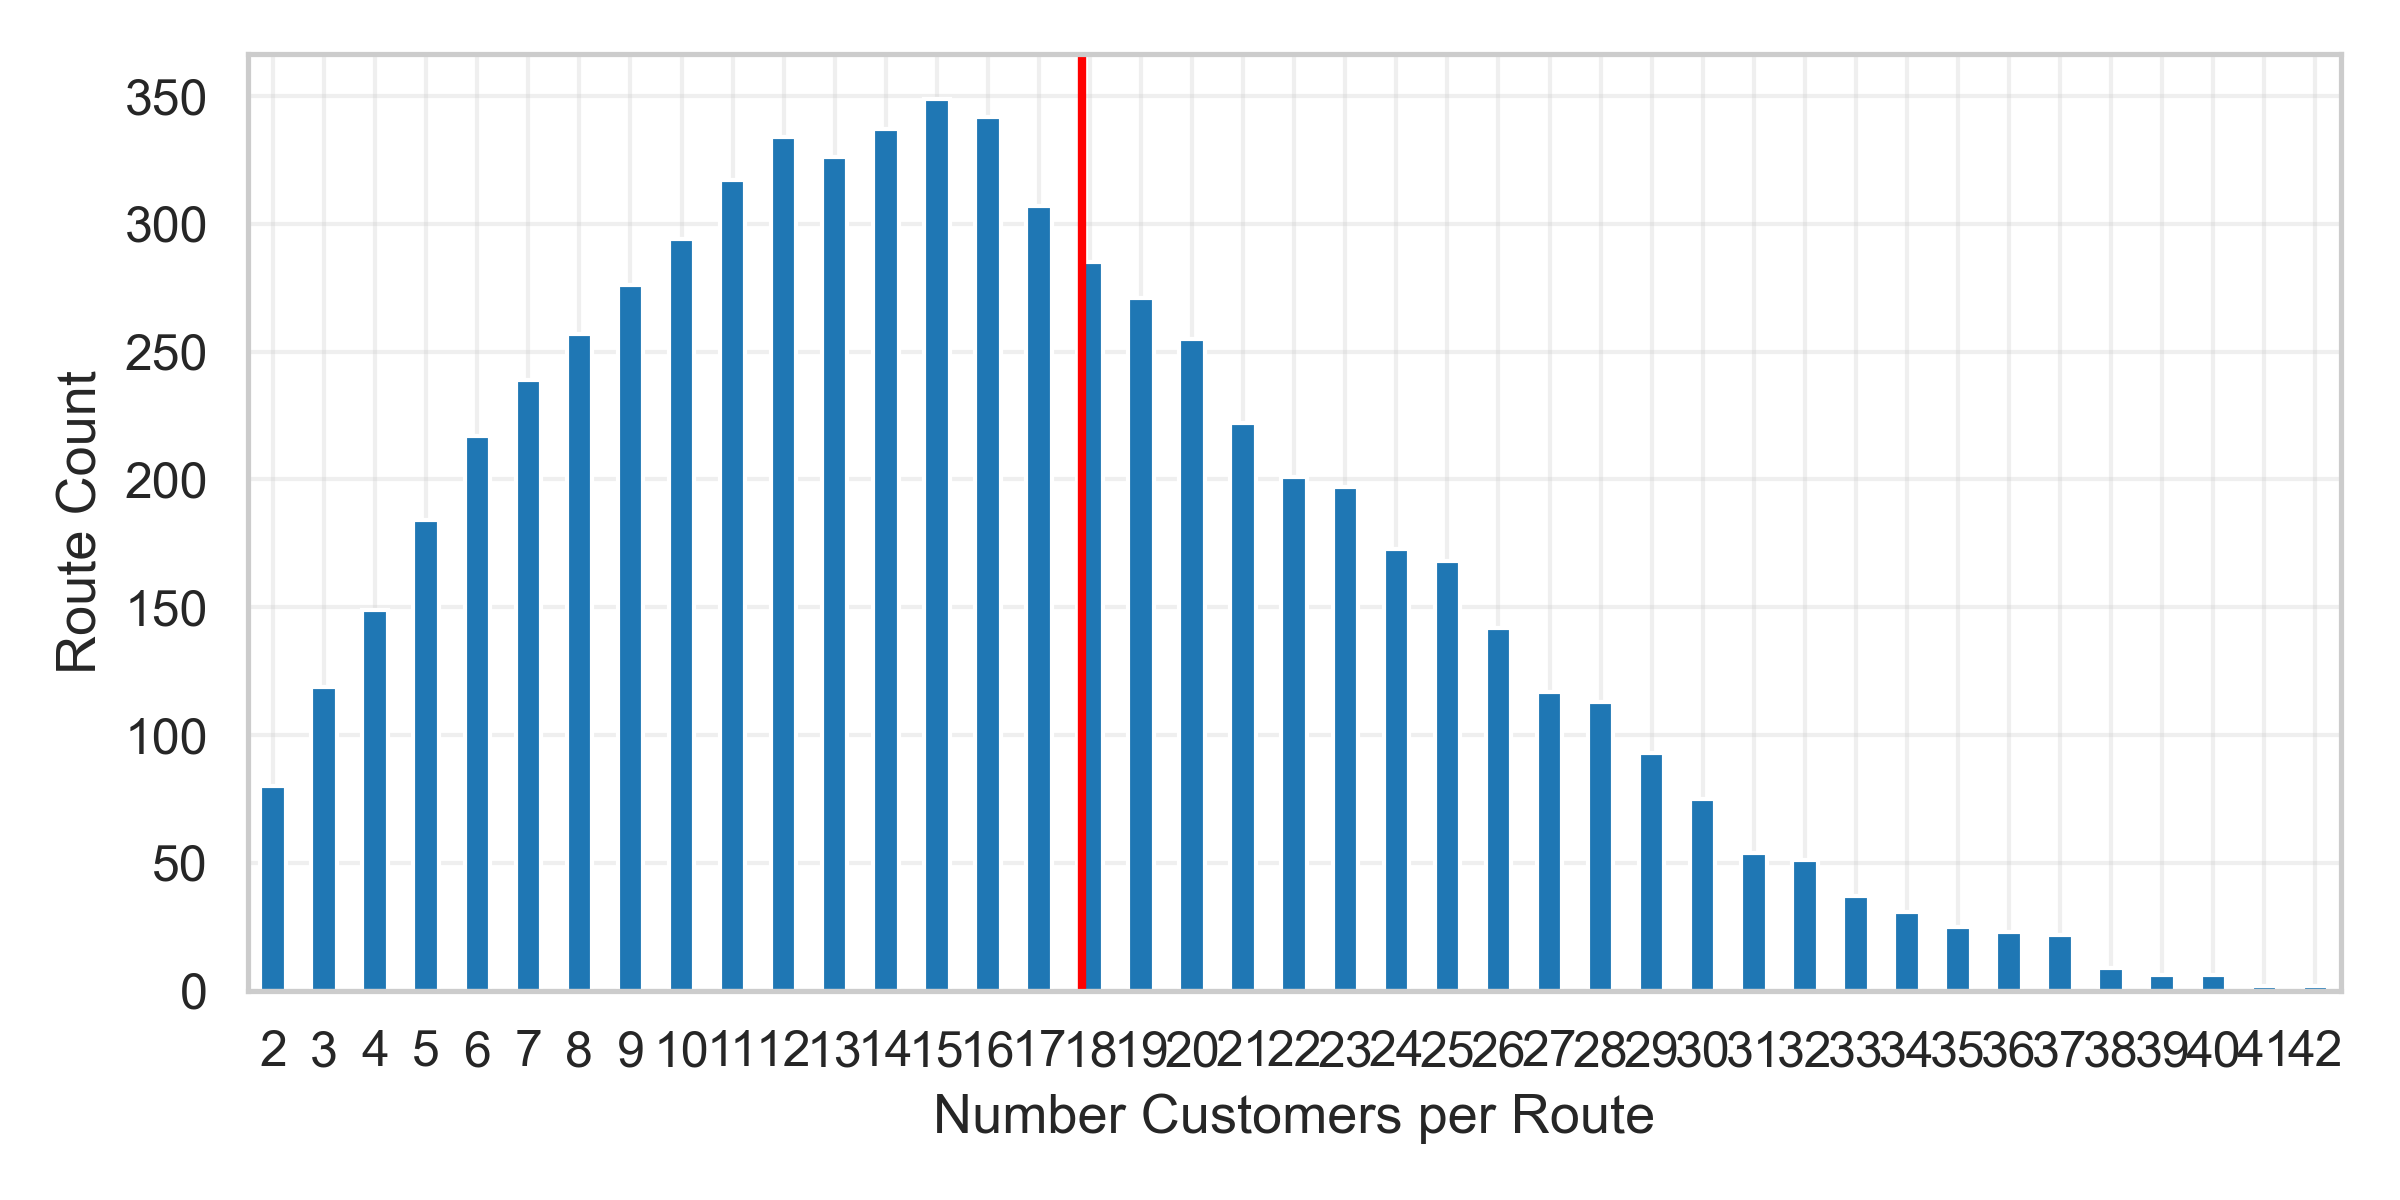
\includegraphics[width=\linewidth]{pictures/dataset_structure/no_cust_plot_RandomData_1_1_1_10.png}
        \caption{Dataset RD-1-1-1-10}
        \label{fig:ds-a-krebs_lop}
    \end{subfigure}%
    \begin{subfigure}[t]{.5\textwidth}
        \centering
        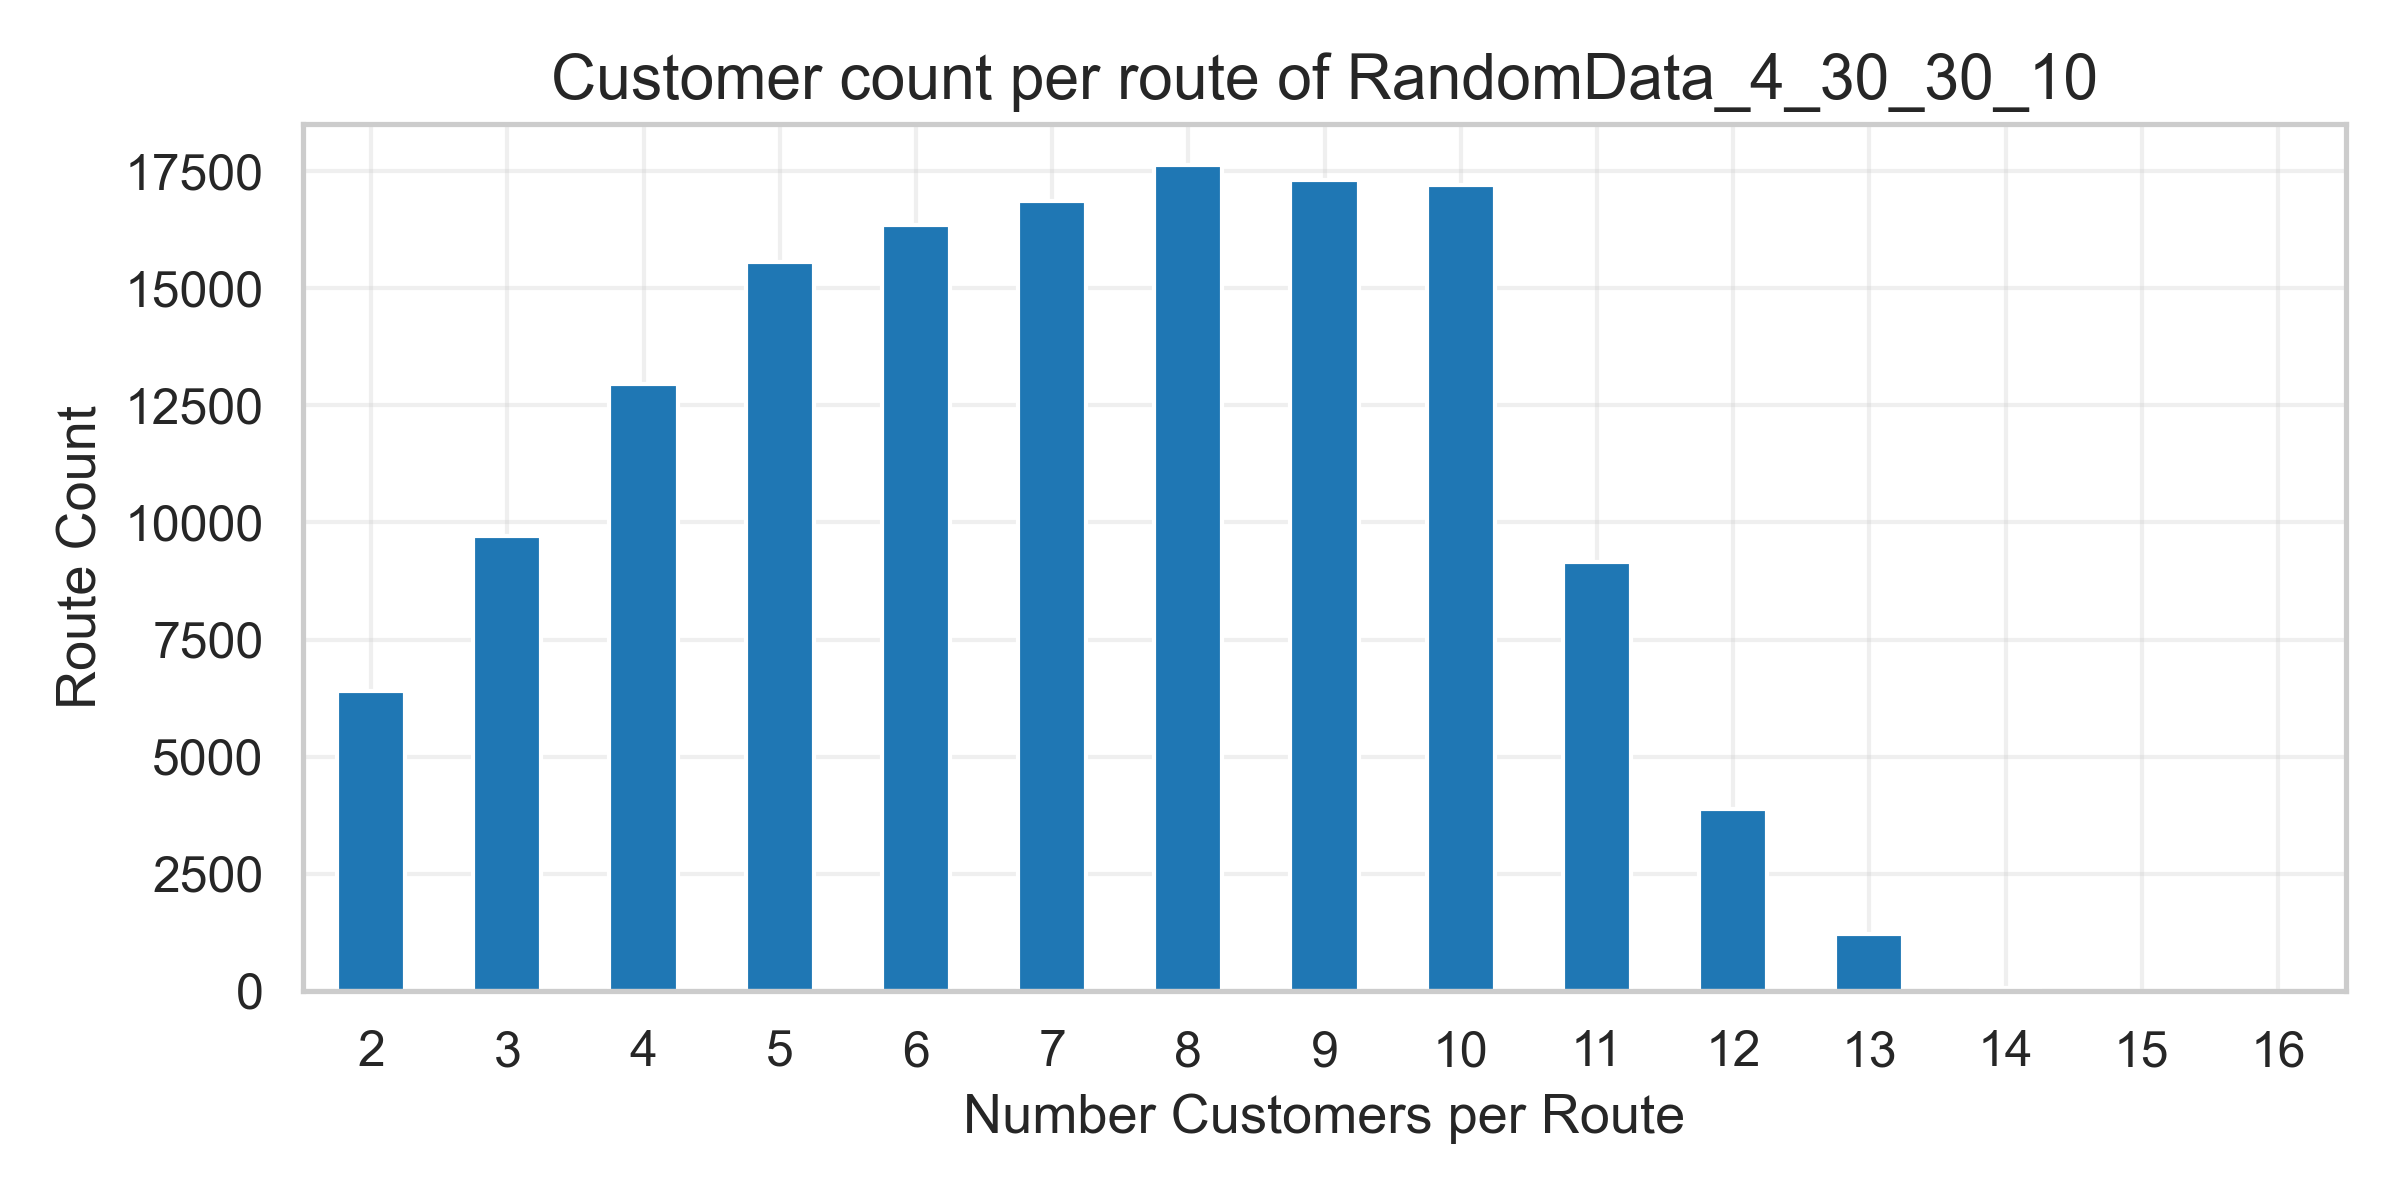
\includegraphics[width=\linewidth]{pictures/dataset_structure/no_cust_plot_RandomData_4_30_30_10.png}
        \caption{Dataset RD-4-30-30-10}
        \label{fig:ds-b-krebs_luf}
    \end{subfigure}
    \caption[Comparison of the distributions of route lengths between the random datasets of \krebsADataSetText and \gendreauDataSet.]
    {Comparison of the distributions of route lengths between the random datasets of \krebsADataSetText and \gendreauDataSet. The red vertical line indicates the average number of customers.}
    \label{fig:route_cust_no_krebs_new}
\end{figure}

\subsubsection{Save retrieval strategy}

Constructing the different save-strategy datasets was more complex due to the longer runtime of the \gls{CP} solver and the undefined
handling of \textit{Invalid} and \textit{Unknown} loading statuses. Subsection~\ref{subsec:challenges_krebs_save} examines these
challenges in more detail. The branch-and-cut results are shown in Table~\ref{tab:bc_results_krebs}, while
Table~\ref{tab:saved_instances_krebs} presents the generated save-strategy datasets.

\begin{table}[ht]
    \centering
    \small
    \begin{tabular}{l c c c c c c }
        \toprule
        Name           & Sets                 & Routes & Routes Len = 2 & Balance   & Rel. Vol & Rel. Mass \\
        \midrule
        KS-Complete-WS & \multirow{3}{*}{Yes} & 261989 & 220860         & 92.4/7.6  & 0.18     & 0.20      \\
        KS-Trimmed-WS  &                      & 41337  & 208            & 52.1/47.9 & 0.58     & 0.63      \\
        KS-Shrunken-WS &                      & 56962  & 15833          & 65.3/34.7 & 0.43     & 0.48      \\        \midrule
        KS-Complete    & \multirow{3}{*}{No}  & 256786 & 220860         & 94.3/5.7  & 0.16     & 0.19      \\
        KS-Trimmed     &                      & 36134  & 208            & 59.6/40.4 & 0.54     & 0.61      \\
        KS-Shrunken    &                      & 51759  & 15833          & 71.8/28.2 & 0.39     & 0.46      \\

        \bottomrule
    \end{tabular}
    \caption{Save strategy train datsets from \krebsADataSet.}
    \label{tab:saved_instances_krebs}
\end{table}

The “Complete” datasets are dominated by routes with two customers, resulting in strongly imbalanced datasets. Consequently,
only the modified datasets, either shrunken or trimmed, are used for model training. However, the trimmed dataset is excluded
from further analysis, as it cannot predict feasible routes with two customers, given that only infeasible tours of this route
length are contained within it and due to the performance issues descibed in Section~\ref{sec:dataset_selection}.

\subsubsection{Dataset Selection}

To identify the best dataset for training, cross-performance metrics between all datasets are compared. However,
as only one save-strategy dataset is considered, no cross-consolidation results need to be excluded. For all datasets,
the drop set DS-50-4 is adopted, since model performance was generally worse due to the high variability (noise) among datasets.
\parbreak
[Insert here: boxplot and table showing the classification performance across datasets.]
\parbreak
Based on these results, the final selected model will be stated and discussed below.

\section{Generalize \gendreauDataSetText models}
\label{sec:krebs_data_pretrained_models}

Two alternatives emerge for this variant. On the one hand, the best model type and corresponding dataset can be selected
from the computational study of the \gendreauDataSetText~(see Section~\ref{sec:comparison_ils_variants}). On the other hand, the
best model type and dataset can be determined by comparing the performance across all four \krebsADataSetText training datasets introduced in the previous section.
As the second alternative combines the strategies of using the same model configuration and adapting it to new datasets, it is
only examined if the best variant–model–dataset combinations identified in Section~\ref{sec:comparison_ils_variants} yield good
results for other \gls{3L-CVRP} datasets. To reduce the computational runtime, only the two best performing variants, NoClassifier
and SpeedUp, are selected (see Table~\ref{tab:final_best_results_gendreau}). The following configurations are chosen based
on the results of all classifier variants compared in Section~\ref{sec_final_comparison_results}.

\begin{table}[ht]
    \centering
    \small
    \begin{tabular}{l c c  }
        \toprule
        Variant      & Model Type & Dataset        \\
        \midrule
        SpeedUp      & XGB        & GD-Shrunken-WS \\
        NoClassifier & -          & -              \\
        \bottomrule
    \end{tabular}
    \caption{Variant configuration for generalization of \gendreauDataSetText results.}
    \label{tab:model_configuration_krebs}
\end{table}

\gls{XGB} was chosen as model type, as it achieved slightly better results
regarding rejection rate and number of iterations, and to increase overall comparability.
The dataset GD-Shrunken-WS minimizes the rejection rate and maximizes the number of iterations for the SpeedUp variant.

\section{Results}
\label{sec:results_krebs}
As shown in Section~\ref{app:sec:krebs_computationally_challenges}, the computation of \krebsADataSetText instances comprises
challenges. Therefore, the algorithmic design is changed. As the computation of the start solution takes averagely \textcolor{red}{1000000000000 seconds}
during the B\&C algorithm (20 seconds for the \gendreauDataSetText), much longer running times are needed for the \gls{ILS} algorithm.
Every instance is only run once. Furthermore, the time limit for one instance
is dependent, if the startsolution is given or will be computed during the algorithm. The start solutions are taken from the branch-and-cut
results (see Section~\ref{tab:bc_results_krebs}). Also it is reevaluated, if the parameter UseFilterStartSolution has a positive effect
for instances demanding much longer computation time for the constructive.



\parbreak
Here are the reuslts for the differnt models and combinations of options, to use or not to use the the filter start solution or the given start solution.

\begin{table}[ht]
    \centering
    \small
    \begin{tabular}{l c c c c }
        \toprule
        Approach                        & $T$                  & Startsolution                    & Variant               & UseFilter \\
        \midrule
        \multirow{3}{*}{Specialization} & 1 h                  & Given                            & SpeedUp/ NoClassifier & False     \\\cmidrule(lr){2-5}
                                        & \multirow{2}{*}{2 h} & \multirow{2}{*}{ModifiedSavings} & SpeedUp/ NoClassifier & False     \\
                                        &                      &                                  & SpeedUp               & True      \\ \midrule
        \multirow{3}{*}{Generalization} & 1 h                  & Given                            & SpeedUp/ NoClassifier & False     \\\cmidrule(lr){2-5}
                                        & \multirow{2}{*}{2 h} & \multirow{2}{*}{ModifiedSavings} & SpeedUp/ NoClassifier & False     \\
                                        &                      &                                  & SpeedUp               & True      \\
        \bottomrule
    \end{tabular}
    \caption[Final configurations for computation of \krebsADataSetText dataset.]{Final configurations for computation of \krebsADataSetText dataset. $T$ stands for Time limit and UseFilter defines the usage of
        filter feasibility check in constructive heuristic}
\end{table}
